\chapter{基于贝叶斯不确定性估计的Med-VQA}
贝叶斯不确定性估计以及贝叶斯神经网络的应用领域十分广泛,不但可以应用于传统的分类和回归任务的学习以及预测,还可以通过学习给定状态下行动的概率分布来学习强化学习问题中的最优策略,
也可以通过将从一个任务中学到的后验分布作为另一个相关任务的先验分布从而将知识从一个任务转移到另一个任务实现迁移学习。最为特殊的是,贝叶斯神经网络可以用来估计
模型预测的不确定性,这在一些具有极高不确定性量化需求的任务中具有十分重要的价值。
%
\section{贝叶斯神经网络}
\subsection{贝叶斯神经网络简介}
传统深度神经网络中的权重参数通常采用点估计的形式,即在训练完成后网络中的权重参数是一个固定值,根据Blundell等人\cite{blundell2015weight}提出的理论,这样的网络忽略了权重中的不确定性,会造成网络对自身预测的“过度自信”\cite{shridhar2019comprehensive}。针对这个问题,Blundell等人提出了一种
贝叶斯神经网络(Bayes neural network,BNN)模型。与普通点估计神经网络不同的是,该BNN的权重是一个概率分布,从而通过权重给深度网络引入了不确定性。这样网络就可以通过权重不确定性来估计自身预测的不确定性。
这些权重的值,也就是权值分布的后验参数可以通过贝叶斯反向传播算法(Bayes by backprop,BBB)学习得到。图\ref{BNN}展示了BNN和传统神经网络的区别。
\begin{figure}[htbp]
	% 图片居中(列居中对齐)
	\centering	
	% 包含当前路径下的Fig文件夹的图片文件
	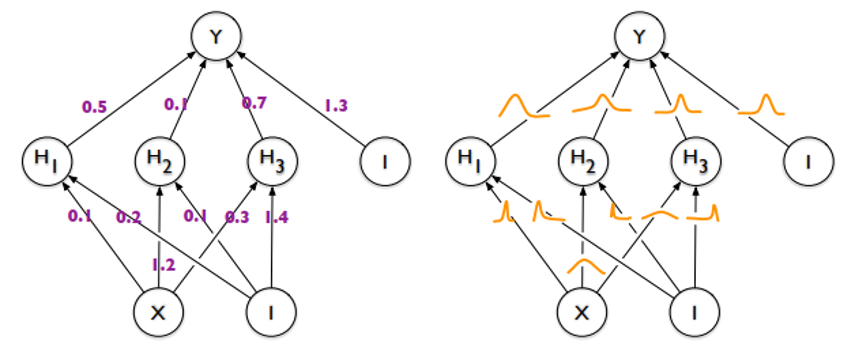
\includegraphics[width=0.9\textwidth]{Fig/myfig/chapter4/BNN.png}  %scale = 0.3
	% 添加标签one_DFUAV以及图标题“XXX”,引用某图时使用\ref{xxx},其中xxx就是标签,图编号是自动生成的。
	\caption{\label{BNN}贝叶斯神经网络} 
\end{figure}

相比传统采用点估计形式的神经网络,BNN具有明显优势。一是通过引入权值的概率分布,BNN可以看作是许多个神经网络的集成,这些集成模型的预测差异可以视为
预测的不确定性。这种不确定性估计的方式也可以用Droppout进行近似模拟\cite{gal2016dropout},通过局部失活后再集成各个网络可以得到更可靠的预测。另一方面,研究证明,贝叶斯方法比最大似然估计更适合于小样本数据建模\cite{mcneish2016using}。
在BNN中,权重参数的后验分布是通过先验和似然的乘积获得的,因此可以通过先验分布将先验信息包含到模型中,这就类似于给模型做了一个正则化。在样本数据较少的情况
下,先验分布可以在计算后验分布时发挥着重要作用,使得贝叶斯方法在小样本情况下仍然能够很好地收敛\cite{mcneish2016using}。因此,通过在权重上设置先验分布,
可以实现对权重的正则化,从而降低网络在小样本训练下的过拟合风险\cite{welling2011bayesian}。

\subsection{局部BNNs与全局BNNs}
局部使用贝叶斯神经网络(L-BNNs)和全局都使用贝叶斯神经网络(G-BNNs)是贝叶斯神经网络的两种不同的应用形式。局部使用贝叶斯神经网络通常是指仅在神经网络的某些层
中使用贝叶斯神经网络,而其他层则采用传统的深度神经网络。Pang等人的研究表明\cite{Pang_Cheng_Hu_Liu_2021},这种方法不但可以提供与全局贝叶斯神经网络近似的不确定性预测性能,
也可以同时帮助解决神经网络的过拟合问题,并提高神经网络的泛化能力。总的来说,全局使用贝叶斯神经网络可以更好地建模模型的不确定性,并且在训练数据不足是仍然具有较好的预测性能,
但伴随着采样率的提升,全局BNN计算成本往往十分高昂,需要几何倍的训练时间和更多的算力资源,使用效率显著降低。
并且在遇到具有较多层数的深度网络或者模块众多的复杂网络时,全局采用贝叶斯神经网络结构不但会增加训练难度,网络的可解释性也会进一步下降。
这时采用局部BNN的策略是一种更为有效的不确定性预测方案,其区别如表\ref{bnn-bnnlr}所示。
\begin{table}
	\caption{\label{bnn-bnnlr}BNN与全局BNN的区别}
	\centering
	\small % 调整表格字号
	\begin{tabular}{c|ccccc}
        \hline 网络结构 & 权重参数形式 & 不确定性估计范围 & 计算效率 & 计算成本 &实用性\\
        \hline G-BNNs & 概率分布 & 全面 & 低 & 高 & 较差\\
		L-BNNs & 确定值\&概率分布 & 局部 & 高 & 低 & 较好\\
        \hline 
        \end{tabular}
\end{table}	
由此,全局的贝叶斯神经网络结构更适合用在一些轻量网络从而获得网络的全局不确定性估计的能力,当涉及复杂的深度神经网络模型,由于网络认知不确定性的前向传播特性\cite{gal2016dropout},使用局部的贝叶斯神经网络进行不确定估计可以在一定程度上替代对其进行全局估计。

\section{用于视觉问答不确定估计的BNNs}
\subsection{网络搭建}
通常参考的是点估计神经网络中的感知机结构,将采用点估计的全连接层替换为BNN结构,通过计算输出的后验分布来预测分类结果以及不确定性。受Zhijie Deng等人\cite{deng2021libre}将局部BNN采样结构用于网络对抗攻击检测的启发,
在Med-VQA问题中,由于与输入图像以及问题相关词向量在经过训练后会具有某种语义关联,低维空间上表现为具有较短的余弦距离。其输出的不确定性往往意味着输入也带有极大的不确定性,所以在语义空间中,
不确定估计往往评估的是语义特征的区分度,高不置信情况下网络提取到的语义特征往往也是无空间关联的,所以采用如\ref{bnn-sublayer}的思想重新设计一个可以预测MEMSA模型预测不确定性的网络结构.
\begin{figure}[htbp]
	% 图片居中(列居中对齐)
	\centering	
	% 包含当前路径下的Fig文件夹的图片文件
	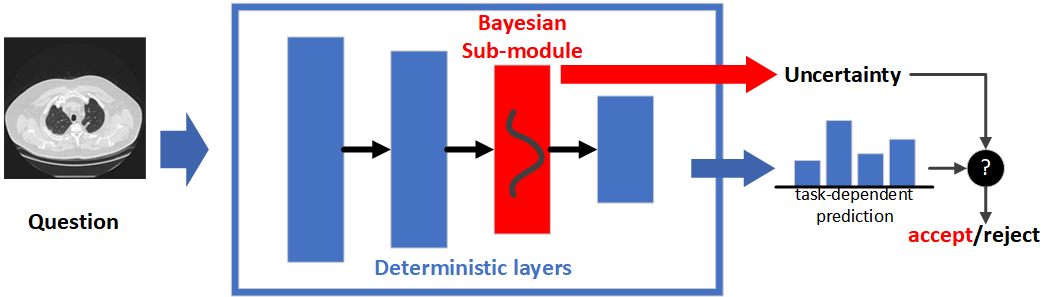
\includegraphics[width=0.9\textwidth]{Fig/myfig/chapter4/bnn-sublayer.png}  %scale = 0.3
	% 添加标签one_DFUAV以及图标题“XXX”,引用某图时使用\ref{xxx},其中xxx就是标签,图编号是自动生成的。
	\caption{\label{bnn-sublayer}局部不确定估计的BNN模型结构} 
\end{figure}

如图\ref{memsabnns}新的MEMSA-BNNs在原模型中最后用于预测的多层感知机网络替换成了多层全连接形式的贝叶斯神经网络结构,此处定义其为BMLP(Bayes Multilayer Perceptron)其作用也是对MEMSA提取到的融合特征进行学习和分类。不同的是BMLP可以依据先验分布形式
对融合特征进行蒙特卡洛采样,从而得到众多子网络,通过这些子网络预测出的结果以及后验分布形式估计预测的不确定性。
\begin{figure}[htbp]
	% 图片居中(列居中对齐)
	\centering	
	% 包含当前路径下的Fig文件夹的图片文件
	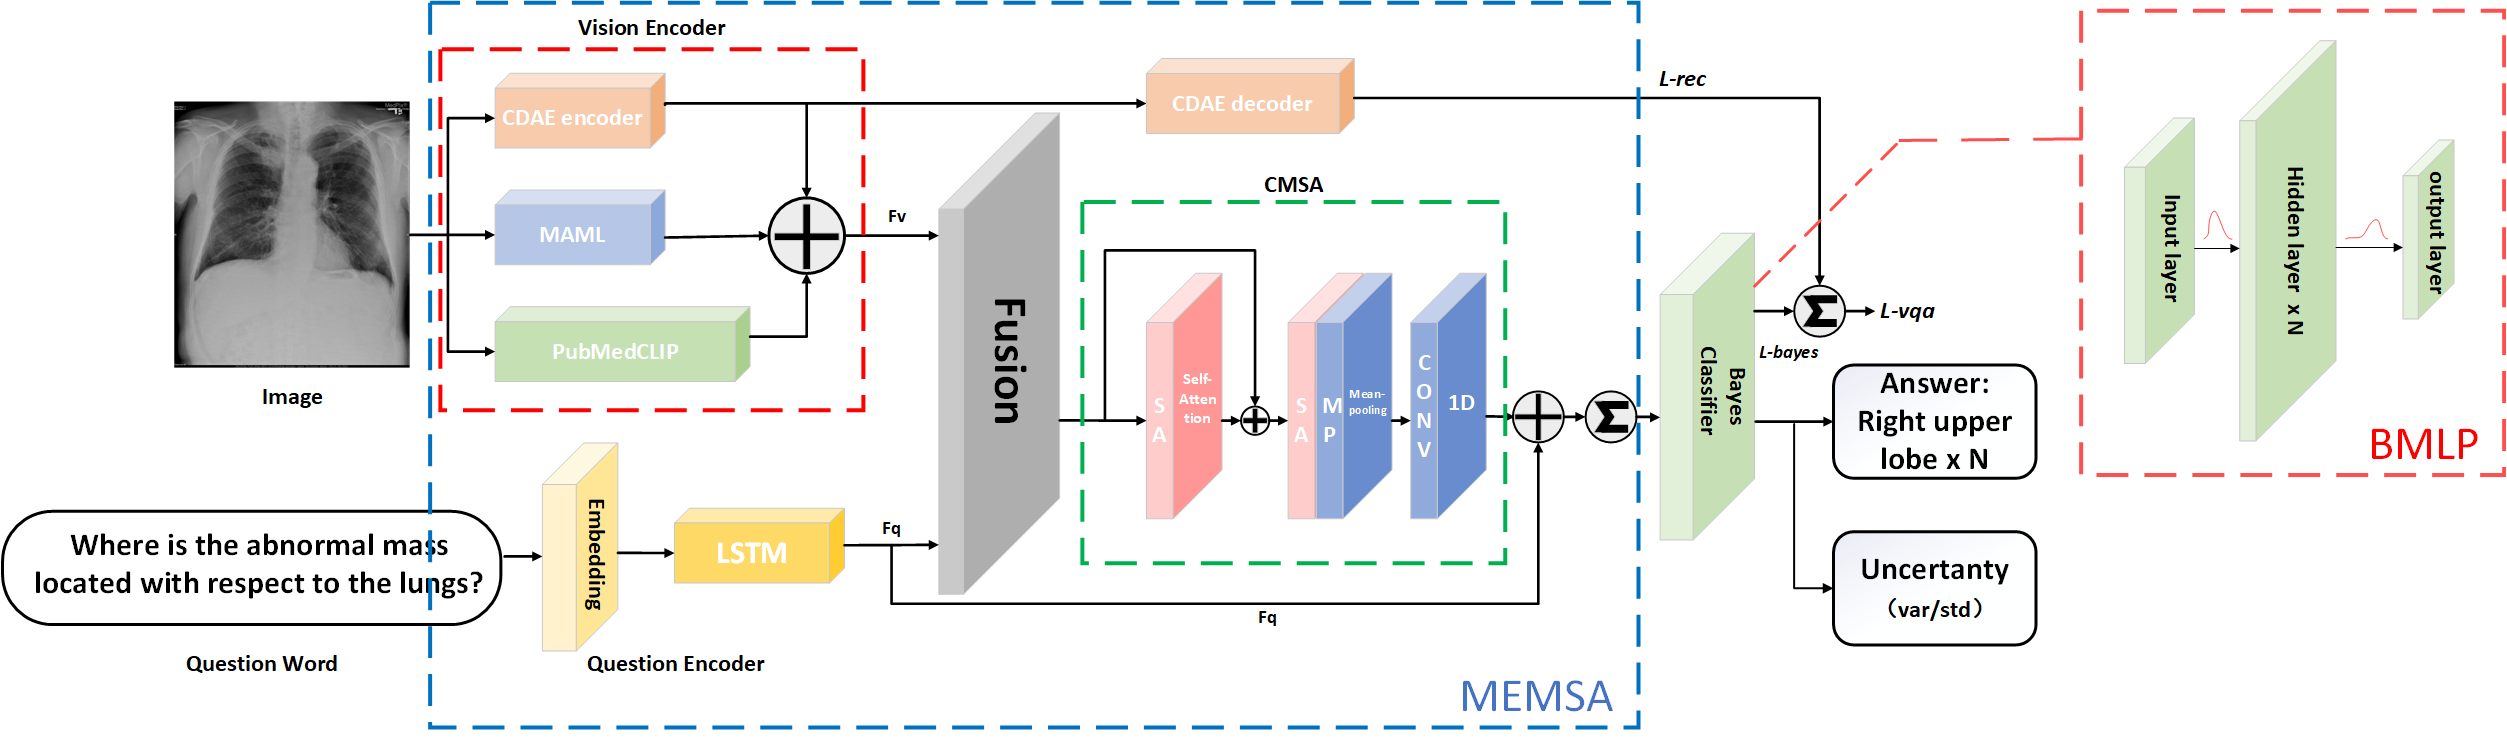
\includegraphics[width=1\textwidth]{Fig/myfig/chapter4/memsabnns.png}  %scale = 0.3
	% 添加标签one_DFUAV以及图标题“XXX”,引用某图时使用\ref{xxx},其中xxx就是标签,图编号是自动生成的。
	\caption{\label{memsabnns}MEMSA-BMLP模型} 
\end{figure}
\subsection{先验分布和后验分布选择}
BNN中先验分布和后验分布地选择往往直接影响模型的性能。先验的选择应该反映设计者对模型的认识以及对模型参数分布的事先预测,例如预测模型经过训练哪些参数更可能接近零,哪些参数可能是正数等等。
先验分布应该尽量简单以避免过拟合,常用的分布有高斯分布或者拉普拉斯分布,针对实际问题,可以采用交叉验证或者网格搜索来评估不同的先验分布和后验分布,以选择最佳的组合。

依据对觉大多数的自然数据的初始分布统计规律,Blundell等人\cite{blundell2015weight}建议将混合高斯分布作为权值的先验分布,该混合高斯由多个高斯密度按照比例混合而成,其中各个高斯密度的均值为0,但方差不一致。
具体来说,该混合高斯先验分布的表达式\eqref{mixgaosi}为:
\begin{equation}
	\label{mixgaosi}
	P(\mathrm{w})=\prod_j \pi N\left(w_j \mid 0, \sigma_1^2\right)+(1-\pi) N\left(w_j \mid 0, \sigma_2^2\right)
\end{equation}
公式中$w_j$是网络中的第j个权值,$N\left(w_j \mid 0, \sigma_1^2\right)$是$w_j$处均值为$\mu$,标准差$\sigma$为的高斯密度。该混合高斯的第一个混合成分的标准差一般要大于第二个成分的标准差($\sigma_1 > \sigma_2$),
这样才能提供比普通高斯先验更重的尾部。第二个混合成分的标准差则要求远小于1,从而使得许多先验权值可以落在零附近,这一种更集中个高斯形式往往更有利于网络学习参数的后验分布形式。除此之外,所有的先验参数在所有权值之间是相同的,这样可以避免要事先对这些权值进行先验优化。本文同样采用了这个混合高斯分布。其中,
第一个混合成分的标准差$\sigma_1$设置成了0.1,第二个混合成分的标准差$\sigma_2$设置成了0.0001。两个高斯间比例权重系数$\pi$设置成了0.5。

本文尝试了各种先验参数的组合并通过实验效果得出了这一最优化参数组合。尝试的先验有:$\sigma_1$(0.1、0.5),$\sigma_2$(0.001、0.0005、0.0001)以及$\pi$(0.25、0.5、0.75)虽然可以让先验分布参数跟随网络参数一起优化,
但这样做通常无法提升模型性能,反而容易导致训练收敛变得缓慢,陷入局部最小值以及导致交差的性能。因此将该先验分布的参数设置为超参数的形式。本文借鉴了Blundell等人的做法,将权值的变分后验分布设置为协方差矩阵,该协方差矩阵同时也是一种对角矩阵的高斯分布形式,
这个分布的均值和标准差即为待优化参数,相比同样结构的点估计全连接神经网络,BNN的待优化参数量要增加一倍以上。

\section{网络训练}
\subsection{贝叶斯反向传播算法}
贝叶斯反向传播算法BBB是一种使用贝叶斯推断来进行神经网络训练的方法,与传统的反向传播算法相比,BBB不仅可以优化神经网络中的权重,
还可以通过计算权重的后验分布来考虑权重的不确定性。为了计算BNN中每个权值的分布,需要通过给定数据来计算权值的后验分布,即$P(w|D)$。
但权值的后验分布形式一般都十分复杂,其解析形式很难直接计算,因此学者们提出了很多对权值的后验分布进行逼近的近似化方法。其中,Hinton、VanCamp\cite{hinton1993keeping}和Graves等人\cite{graves2011practical}提出
通过变分近似来估计权值的真实后验分布。详细地说,为神经网络中的每个权值形式设定一个易于处理的变分后验分布$q(w|\theta)$,其中$\theta$是变分参数。
然后再通过最小化$P(w|D)$和$q(w|\theta)$之间的KL(Kullback-Leibler)散度,从而使得这些参数的变分后验分布不断逼近真实后验分布。获得
变分后验分布之后,BNN网络中的权值后验分布就可以替换为变分后验分布。$P(w|D)$和$q(w|\theta)$之间的KL散度公式如:
\begin{equation}
	\label{}
	\begin{aligned}
	\mathrm{KL}[q(\mathrm{w} \mid \theta) \| P(\mathrm{w} \mid D)] & =\int q(\mathrm{w} \mid \theta) \log \frac{q(\mathrm{w} \mid \theta)}{P(\mathrm{w} \mid D)} d \mathrm{w} \\
	& =\int q(\mathrm{w} \mid \theta) \log \frac{q(\mathrm{w} \mid \theta) P(D)}{P(\mathrm{w}) P(D \mid \mathrm{w})} d \mathrm{w} \\
	& =\int q(\mathrm{w} \mid \theta)\left[\log P(D)+\log \frac{q(\mathrm{w} \mid \theta)}{P(\mathrm{w})}-\log P(D \mid \mathrm{w})\right] d \mathrm{w} \\
	& =\log P(D)+\mathrm{KL}[q(\mathrm{w} \mid \theta) \| P(\mathrm{w})]-\int P(\mathrm{w} \mid \theta) \log P(D \mid \mathrm{w}) d \mathrm{w}
	\end{aligned}
\end{equation}
因此得到:
\begin{equation}
	\label{}
	\begin{aligned}
	\log P(D)= & \mathrm{KL}[q(\mathrm{w} \mid \theta) \| P(\mathrm{w} \mid D)]-\operatorname{KL}[q(\mathrm{w} \mid \theta) \| P(\mathrm{w})] \\
	& +\int q(\mathrm{w} \mid \theta) \log P(D \mid \mathrm{w}) d \mathrm{w}
	\end{aligned}
\end{equation}
因为$log P(D)$为一个常数,为了最小化$mathrm{KL}[q(\mathrm{w} \mid \theta) \| P(\mathrm{w} \mid D)]$,则需要最小化以下公式:
\begin{equation}
	\label{}
	\mathcal{F}(D, \theta)=\mathrm{KL}[q(\mathrm{w} \mid \theta) \| P(\mathrm{w})]-\int q(\mathrm{w} \mid \theta) \log P(D \mid \mathrm{w}) d \mathrm{w}
\end{equation}
$mathcal{F}(D, \theta)$即为贝叶斯神经网络的损失函数,通过最小化$mathcal{F}(D, \theta)$即可获得变分后验参数$θ$。Neal等人\cite{neal1998view}将这种损失函数称为变分自由能\cite{friston2007variational}
或期望下限\cite{jaakkola2000bayesian}。$mathcal{F}(D, \theta)$的第一项被称为复杂损失项,它依赖于输入的先验分布或者先验知识。第二项被称为似然损失项,它依赖于数据$D$。由于损失函数$mathcal{F}(D, \theta)$
是针对整个数据集的,但通常在神经网络的训练中采用的是小批次随机梯度下降的训练方法。假定数据集$D$被分成M个大小相同的批次,那对于每个批次$D_i$,复杂性损失
项通常需要乘上加权值$1/M$,此时损失函数变为\cite{blundell2015weight}:
\begin{equation}
	\label{}
	\mathcal{F}\left(D_i, \theta\right)=\frac{1}{M} \mathrm{KL}[q(\mathrm{w} \mid \theta) \| P(\mathrm{w})]-\int q(\mathrm{w} \mid \theta) \log P\left(D_i \mid \mathrm{w}\right) d \mathrm{w}
\end{equation}

这样,每个批次的损失之和$\sum_{i}\mathcal{F}\left(D_i, \theta\right)$等于$mathcal{F}(D, \theta)$。此外,Blundell等人\cite{blundell2015weight}还提出了另一种
对复杂性损失项的加权方法:
\begin{equation}
	\label{}
	\mathcal{F}\left(D_i, \theta\right)=\pi_i \mathrm{KL}[q(\mathrm{w} \mid \theta) \| P(\mathrm{w})]-\int q(\mathrm{w} \mid \theta) \log P\left(D_i \mid \mathrm{w}\right) d \mathrm{w}
\end{equation}
其中加权值$pi_i$为:
\begin{equation}
	\label{}
	\pi_i = \frac{2^M-i}{2^M - 1}
\end{equation}

通过上式,可见$\pi_i$随训练而逐渐减小。这种训练方式在初始训练网络时十分有用,因为在刚开始的几个训练批次中,加权值$\pi_i$最大,
因此在两项损失中复杂性损失占主要作用,此时权值变化较少。随着训练次数增大,数据增多以及$\pi_i$逐渐减小,此时数据对权值的更新的影响越来越来大,
相对的,先验的作用越来越小。

对于BNN,想要精确最小化损失$\mathcal{F}(D, \theta)$是不可行的。因此,Blundell等人\cite{blundell2015weight}提出了贝叶斯反向传播算法BBB,通过梯度下降
来求解变分参数$\theta$。首先,通过展开$\mathrm{KL}[q(\mathrm{w} \mid \theta) \| P(\mathrm{w} \mid D)]$这一项,
$\mathcal{F}(D, \theta)$可以化解为:
\begin{equation}
	\label{kl_sandu}
	\mathcal{F}(D, \theta)=\int q(\mathrm{w} \mid \theta)[\log q(\mathrm{w} \mid \theta)-\log P(\mathrm{w})-\log P(D \mid \mathrm{w})] d \mathrm{w}
\end{equation}

然后通过蒙特卡洛采样方法来近似以上期望,即:
\begin{equation}
	\label{mtkl_sample_methoes}
	\mathcal{F}(D, \theta) \approx \sum_{i=1}^n \log q\left(\mathrm{w}^{(i)} \mid \theta\right)-\log P\left(\mathrm{w}^{(i)}\right)-\log P\left(D \mid \mathrm{w}^{(i)}\right)
\end{equation}

其中$\mathrm{w}^{(i)}$代表从变分后验$q(\mathrm{2}) \mid \theta$采样的第$i$个蒙特卡洛样本。在Blundell提出的方法中,变分后验分布被设置为一种
协方差矩阵为对角矩阵的高斯分布。令$\mu$代表该高斯分布的均值,$\sigma$代表该高斯分布的标准差。因为$\sigma$总是非负的,为了保证这一条件
通常将$\sigma$参数化为:
\begin{equation}
	\label{}
	\sigma = \log (1+\exp(\rho))
\end{equation}
输出$\rho$称为标准差参数。此时有变分后验参数$\theta=(\mu,\rho)$。但由于从分布中采样是不可导的,这会导致神经网络无法进行反向传播。这一
问题可以通过采用重参化\cite{kingma2013auto}技巧解决:
\begin{equation}
	\label{}
	\mathrm{w}=\mu+\log (1+\exp (\rho)) * \epsilon, \quad \epsilon \sim N(0, I)
\end{equation}
其中$w$相当于变分分布中采样得到的权值,$\epsilon$是噪声变量,它从标准正态分布中采样得到。由于以上采样过程只涉及线性操作,因此该采样的过程是可导的。
总的来说,BBB中的重参化技术将随机性从权重中移除,使其可以直接计算梯度。这使得BBB能够高效地进行反向传播,并且可以在大型的神经网络中使用。
由此,可以推导出贝叶斯反向传播算法的过程\cite{blundell2015weight}:
\begin{enumerate}
	\item 从标准正态分布中对噪声进行采样:
	\begin{equation}
		\label{}
		\quad \epsilon \sim N(0, I)
	\end{equation}
	\item 从变分后验中对权值进行采样:
	\begin{equation}
		\label{}
		\mathrm{w}=\mu+\log (1+\exp (\rho)) * \epsilon
	\end{equation}
	\item 损失计算:
	\begin{equation}
		\label{}
		f(\mathrm{w},\theta)= logq(\mathrm{w}\mid\theta)
	\end{equation}
	\item 计算损失关于均值的梯度:
	\begin{equation}
		\label{}
		\Delta_\mu=\frac{\partial f(\mathrm{w}, \theta)}{\partial \mathrm{w}}+\frac{\partial f(\mathrm{w}, \theta)}{\partial \mu}
	\end{equation}
	\item 计算损失关于标准差参数的梯度:
	\begin{equation}
		\label{}
		\Delta_\rho=\frac{\partial f(\mathrm{w}, \theta)}{\partial \mathrm{w}} \frac{\epsilon}{1+\exp (-\rho)}+\frac{\partial f(\mathrm{w}, \theta)}{\partial \rho}
	\end{equation}
	\item 更新变分参数:
	\begin{equation}
		\label{}
		\begin{aligned}
		& \mu \leftarrow \mu-\alpha \Delta_\mu \\
		& \rho \leftarrow \rho-\alpha \Delta_\rho
		\end{aligned}
	\end{equation}
\end{enumerate}
其中$\aleph$是学习率。以上步骤仅是一次蒙特卡洛采样训练过程。为了更精准的估计公式\eqref{kl_sandu}的积分,在网络训练过程中往往会进行多次的
蒙塔卡洛采样,计算出多个损失后再求平均。

\subsection{网络预测}
BNN在训练时通过执行贝叶斯反向传播算法,使得权值的变分后验分布不断逼近真实的后验分布。当网络训练完成之后,所得到的变分后验可以近似替代真实后验,之后便能够
对数据进行预测。BNN对数据x的预测公式为:
\begin{equation}
	\label{}
	\begin{aligned}
	P(y \mid x, D) & =\int P(y \mid x, \mathrm{w}) P(\mathrm{w} \mid D) d \mathrm{w} \\
	& =\int P(y \mid x, \mathrm{w}) q(\mathrm{w} \mid \theta) d \mathrm{w}
	\end{aligned}
\end{equation}
其中$P(y|x,D)$是给定权值w时网络的输出。该积分其实等价于对无数个模型做出预测并进行平均。但是在$w$空间上进行的积分一通常是难以计算的,
因此该项积分也通常采用蒙特卡洛方法进行估计近似,故此时BNN的预测公式为:
\begin{equation}
	\label{}
	P(y \mid x, D) \approx \frac{1}{T} \sum_{t=1}^T P\left(y \mid x, w_t\right), \quad w_t \sim q(\mathrm{w} \mid \theta)
\end{equation}
其中$w_t$是从$q(\mathrm{w})\mid\theta$中采样得到的权值,$T$为采样次数,之后取这T次预测的平均作为BNN的输出。这T个预测的
差异就可以视为预测的不确定性,通常采用方差或者标准差对这些差异进行度量。从中可见BNN相当于多个模型的集成,这可以提高网络的泛化能力,减少过拟合的风险。
%
% \subsection{模型复杂度分析}

%
\section{实验结果与分析}
\subsection{模型性能实验}
BNNs针对分类问题有着较为优异的性能,在提供不确定可以有效防止过拟合。如表\ref{mlp2bmlp}是模型在两个不同量级数据集下将局部网络结构中替换成BNNs所取得的性能效果:
\begin{figure}[htbp]
	\begin{minipage}{0.5\linewidth}
		\centering	
		% 包含当前路径下的Fig文件夹的图片文件
		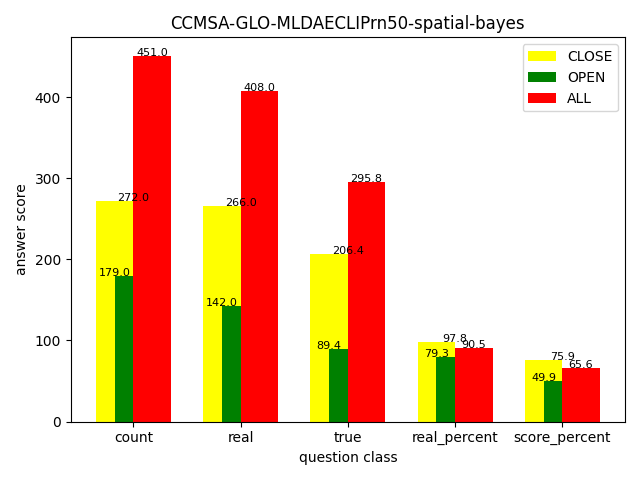
\includegraphics[width=1\textwidth]{Fig/myfig/chapter4/modal_bayes_medrad.png}  %scale = 0.3
		% 添加标签one_DFUAV以及图标题“XXX”,引用某图时使用\ref{xxx},其中xxx就是标签,图编号是自动生成的。
		\caption{\label{modal_bayes_medrad}Med-RAD数据集BMLP性能} 	
	\end{minipage}
	% 图片居中(列居中对齐)
	\begin{minipage}{0.5\linewidth}
		\centering	
		% 包含当前路径下的Fig文件夹的图片文件
		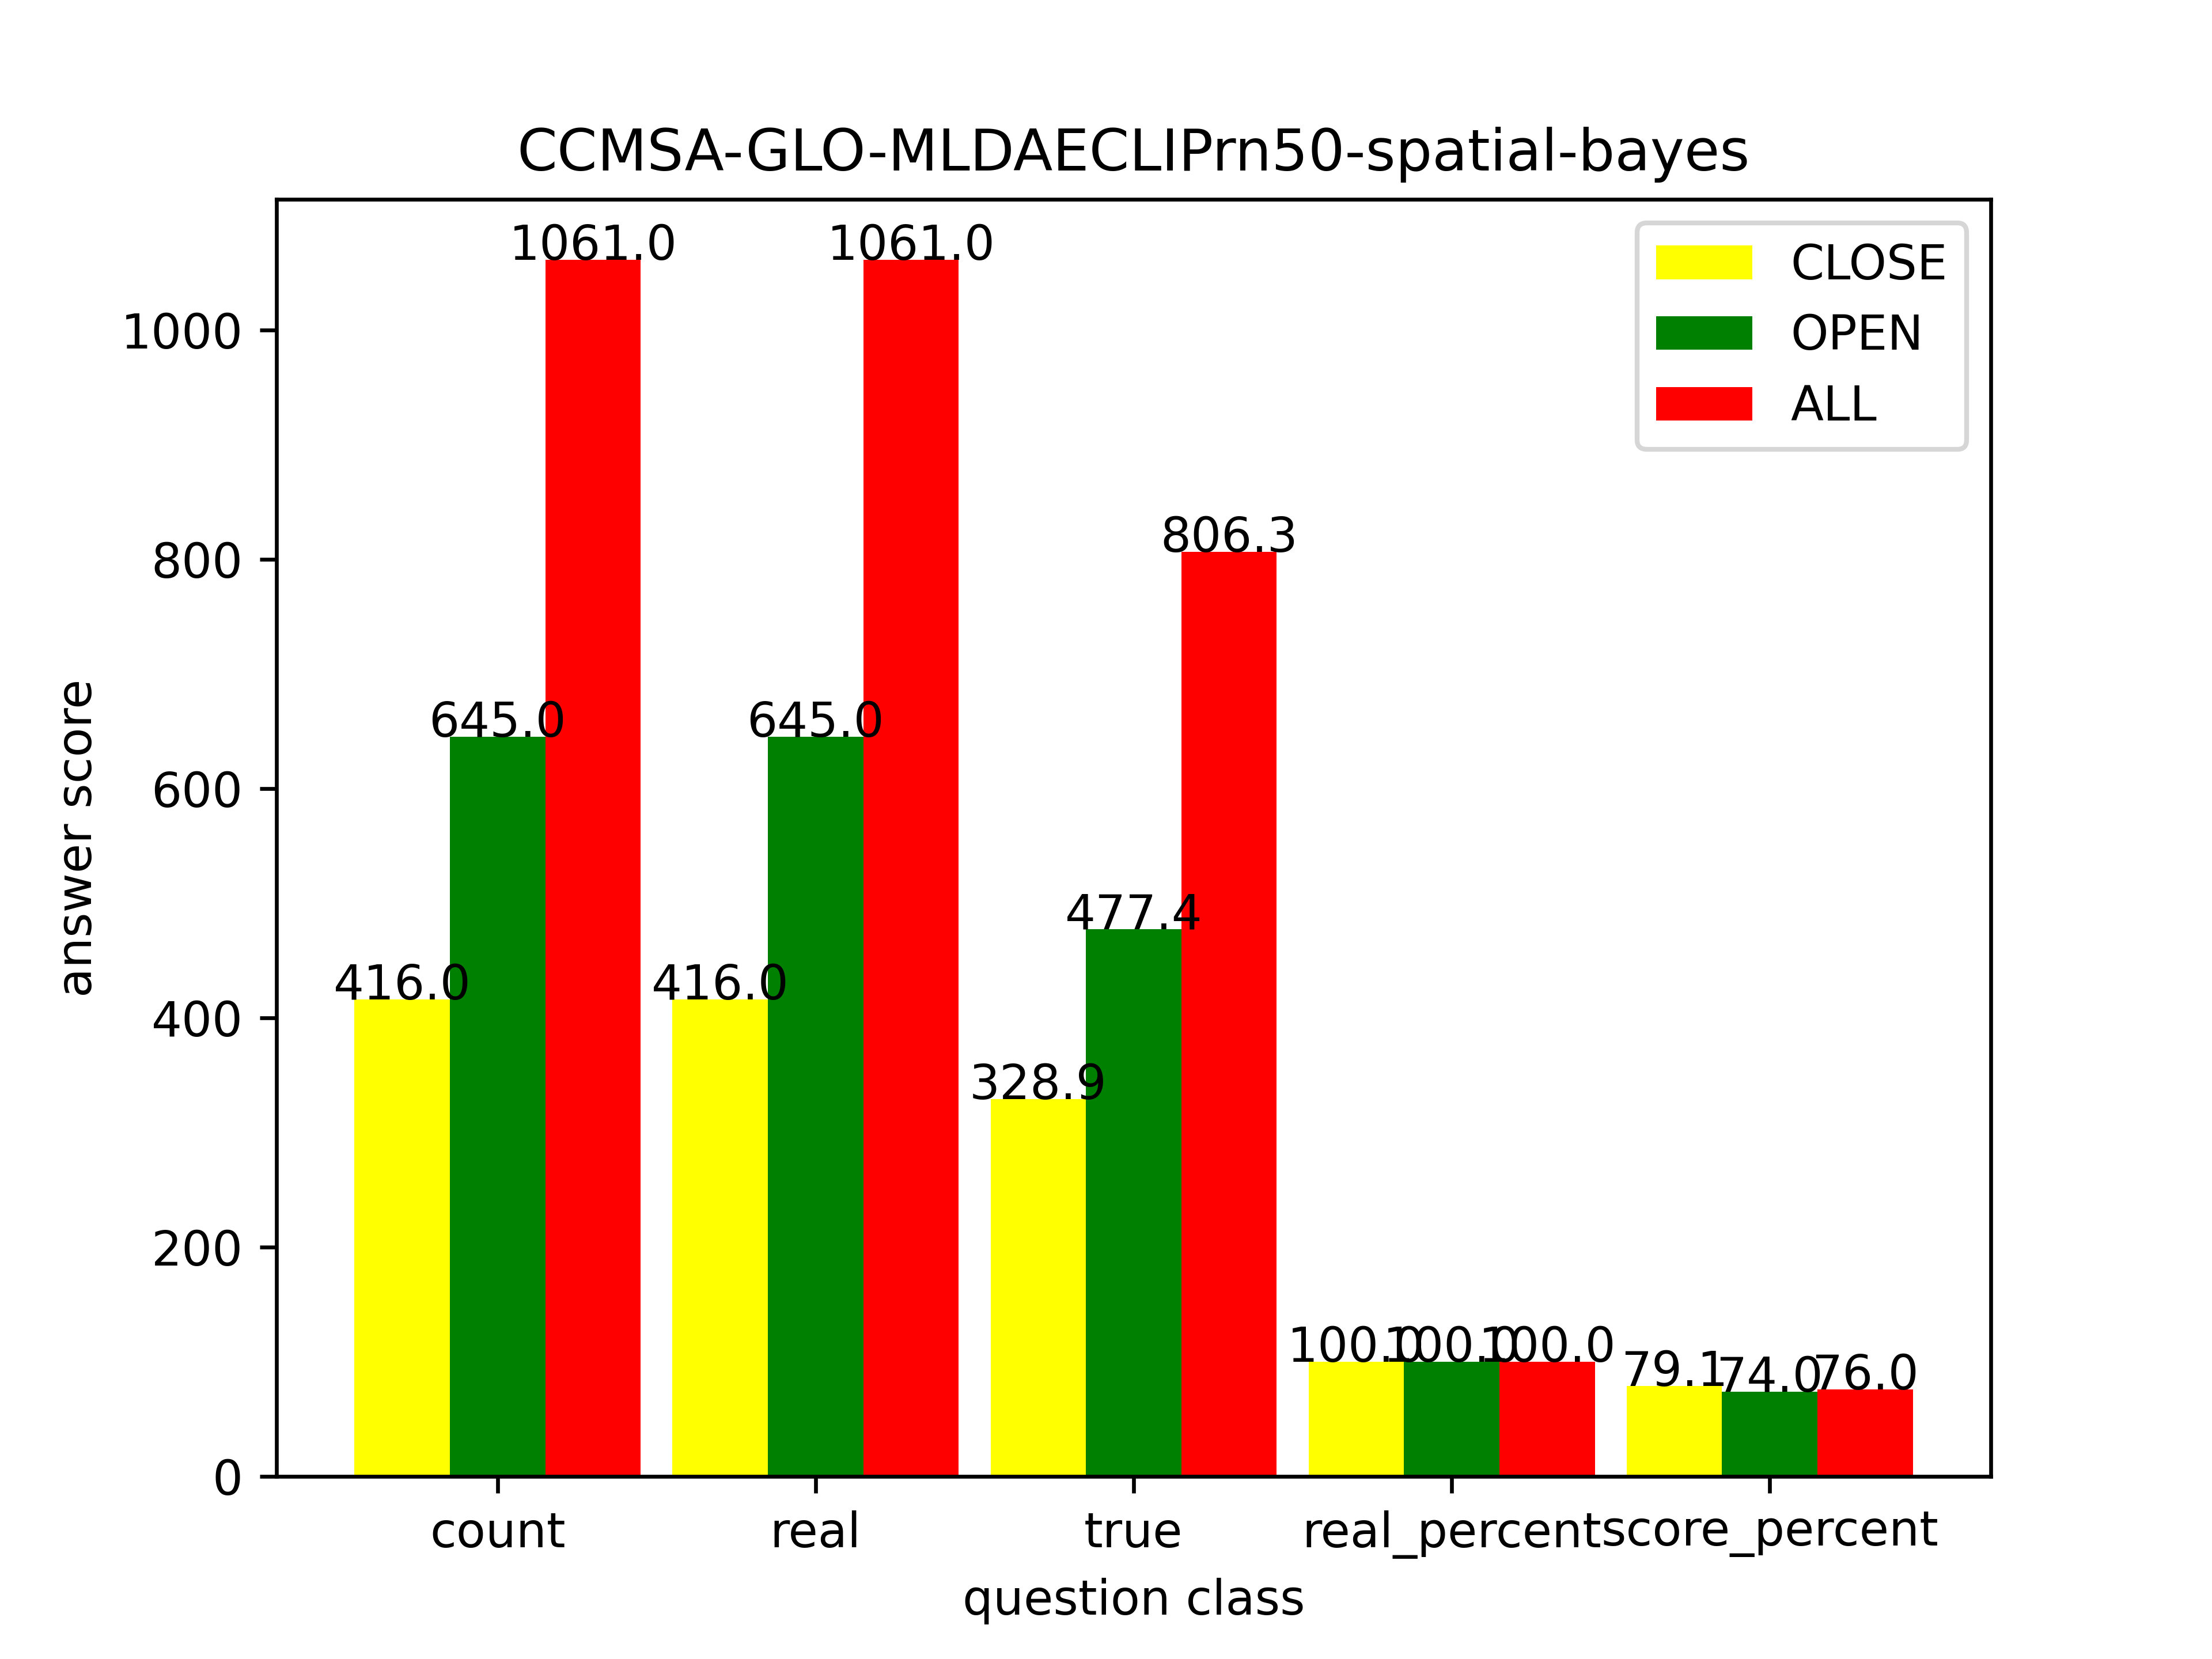
\includegraphics[width=1\textwidth]{Fig/myfig/chapter4/modal_bayes_slake.png}  %scale = 0.3
		% 添加标签one_DFUAV以及图标题“XXX”,引用某图时使用\ref{xxx},其中xxx就是标签,图编号是自动生成的。
		\caption{\label{modal_bayes_slake}SLAKE数据集BMLP模型性能} 	
	\end{minipage}	
\end{figure}

% \begin{figure}[htbp]
% 	% 图片居中(列居中对齐)
% 	\centering	
% 	% 包含当前路径下的Fig文件夹的图片文件
% 	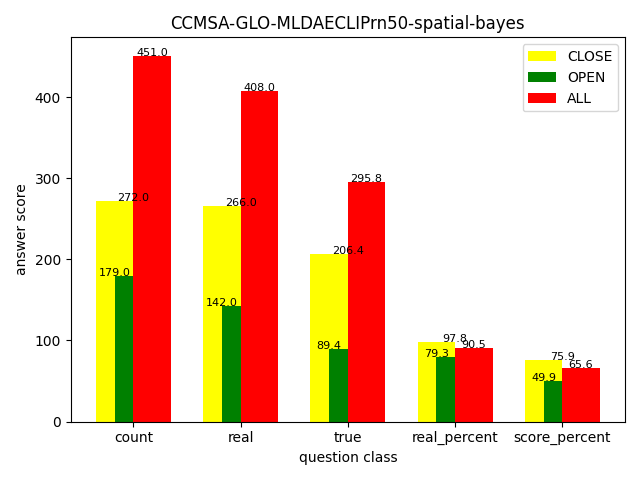
\includegraphics[width=0.9\textwidth]{Fig/myfig/chapter4/modal_bayes_medrad.png}  %scale = 0.3
% 	% 添加标签one_DFUAV以及图标题“XXX”,引用某图时使用\ref{xxx},其中xxx就是标签,图编号是自动生成的。
% 	\caption{\label{bnn-sublayer}BMLP在Med-RAD数据集上的性能表现} 
% \end{figure}
% \begin{figure}[htbp]
% 	% 图片居中(列居中对齐)
% 	\centering	
% 	% 包含当前路径下的Fig文件夹的图片文件
% 	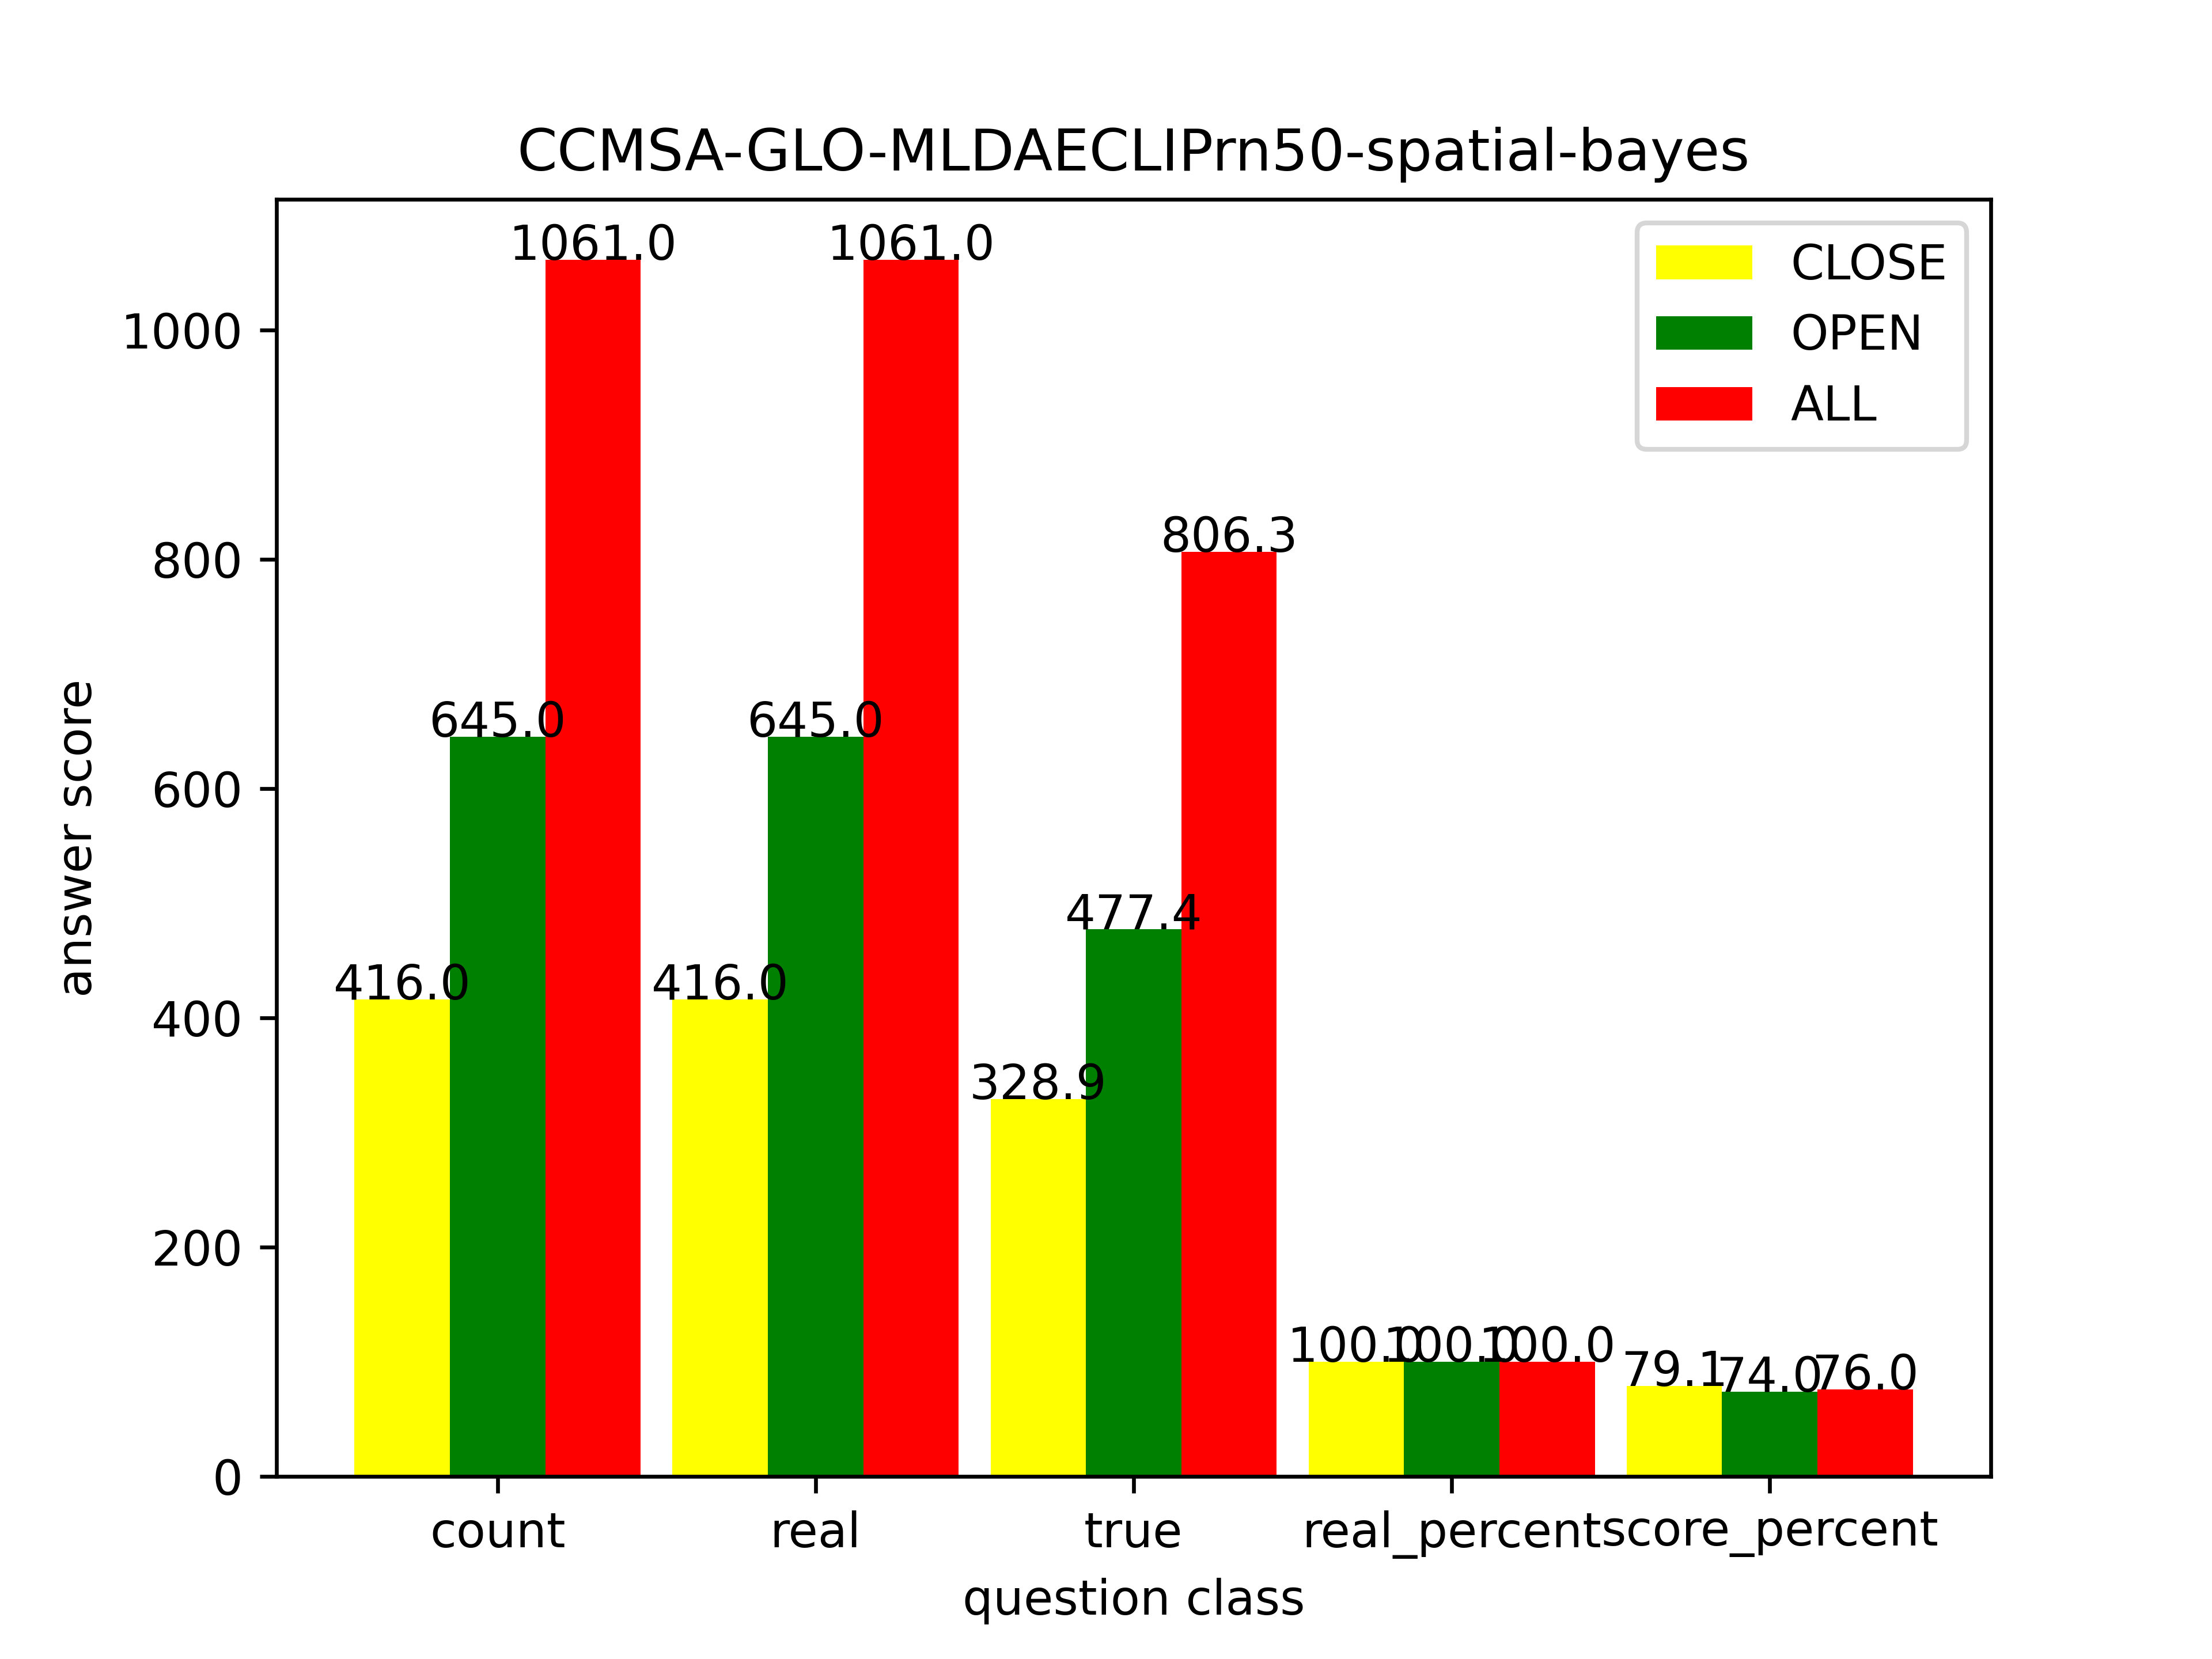
\includegraphics[width=0.9\textwidth]{Fig/myfig/chapter4/modal_bayes_slake.png}  %scale = 0.3
% 	% 添加标签one_DFUAV以及图标题“XXX”,引用某图时使用\ref{xxx},其中xxx就是标签,图编号是自动生成的。
% 	\caption{\label{bnn-sublayer}BMLP在SLAKE数据集上的性能表现} 
% \end{figure}
%
% \begin{table}
% 	\caption{\label{bnn-bnnlr}BNN与全局BNN的区别}
% 	\centering
% 	\small % 调整表格字号
% 	\begin{tabular}{l|l|lll}
% 		\hline Dataset & Methods & Open & Closed & ALL \\
% 		\hline \multirow{2}{*}{Med-RAD} & Ours(no.bnns) & $65.4 \%$ & $77.6 \%$ & $72.7 \%$ \\
% 		& Ours(add.bnns) & $56.4 \% \pm 1.5 \%$ & $73.9 \% \pm 1.1 \%$ & $66.7 \% \pm 1.8 \%$ \\
% 		\hline \multirow{2}{*}{ SLAKE } & Ours(no.bnos) & $76.0 \%$ & $81.7 \%$ & $78.2 \%$ \\
% 		& Ours(add.bnns) & $73.5 \% \pm 1.2 \%$ & $81.7 \% \pm 0.3 \%$ & $76.7 \% \pm 0.9 \%$ \\
% 		\hline
% 	\end{tabular}
% \end{table}
\begin{table}
	\caption{\label{mlp2bmlp}MEMSA使用BMLP和MLP的性能对比}
	\centering
	\small % 调整表格字号
	$$
	\begin{array}{l|l|lll}
	\hline \text { Dataset } & \text { Methods } & \text { Open } & \text { Closed } & \text { ALL } \\
	\hline \multirow{2}{*}{\text { Med-RAD }} & \text { MEMSA-MLP } & 65.4 \% & 77.6 \% & 72.7 \% \\
	% & \text { MEMSA-BMLP } & 51.8 \% & 77.7 \% & 68.4 \% \\
	& \text { MEMSA-BMLP } & 59.1 \% & 74.7 \% & 68.5 \% \\
	\hline \multirow{2}{*}{\text { SLAKE }} & \text { MEMSA-MLP } & 76.0 \% & 81.7 \% & 78.2 \% \\
	& \text { MEMSA-BMLP } & 74.0 \% & 79.1 \% & 76.0 \% \\
	\hline
	\end{array}
	$$
\end{table}

通过上述图表可以发现,在传统点估计模型中引入BNN后,模型用同样的参数去额外拟合不确定性(Uncertainty)会带来精度上的一些损失,
同时由于采用贝叶斯反向传播算法是一种采用变分估计的近似算法,这些误差也会最终对模型的精度造成影响。通过后续的采样率和不确定性测试可知,
这种精度损失和原本数据分布的散度,也就是数据不确定性呈正相关。例如Med-RAD数据集相对SLAKE数据少,所拥有的可预测标签值却是SLAKE数据集的两倍,
在空间中呈现更加分散的分布,BNN在对这类数据进行拟合和预测时往往具有较大的方差,也就是不确定性,进而影响分类性能。
在更小的数据集上,加入贝叶斯分类器也仍然可以取得平均以上的性能,这说明贝叶斯分类器有防止模型过拟合的作用。


\subsection{采样率-不确定性测试实验}
贝叶斯网络的不确定性预测其实本质也来自于多个模型集成的思想。经过对分布的采样获得多个模型预测结果的均值代表模型最终的预测,而方差则代表了其对于预测结果的不确定程度。
方差越大,模型越不置信,而为了保证医学问答场景下的严谨和安全,医学问答模型能够获得对自身结果预测的不确定程度。值得一提的是,这种不确定和传统softmax函数计算出来的输出层概率分布具有不同的含义,softmax由于是
权值固定的点估计网络,softmax经过软归一的出来的概率分布结果也是模型“置信”的,这个分布只和网络对该层的训练有关,另外该层也无法通过重新采样去预测结果。虽然可以用Dropout方法达到近似的效果\cite{},但由于不像BNN具有
先验知识的输入,Drop的输出的不确定性难以从输出中找到预测的实际意义,也就是可解释性低。所以与置信度研究不同,研究BNN在预测Med-VQA中不确定的由来具有十分重要的意义。

由于贝叶斯神经网络是通过不断进行蒙特卡洛下采样来获取网络中的不确定性信息的,图\ref{sample_sum}展示了各采样频率下与模型不确定性估计之间关联,图中横坐标代表预测的问题,
纵坐标代表预测的输出分布。横坐标每个问题的预测轴中黄色部分代表预测正确的次数,蓝色代表非正确预测的次数,轴总高度即采样率,是一个固定值。经过排序且由积分关系可知,整张图中黄色部分的面积占比
代表了模型预测准确率,横坐标两侧全部由黄色和蓝色轴组成的部分是模型对预测做出确定性回答的问题,中间由黄色虚线框选中的蓝黄参半部分即为预测时具有不确定性区间。

\begin{figure}[htbp]
	% 图片居中(列居中对齐)
	\centering	
	% 包含当前路径下的Fig文件夹的图片文件
	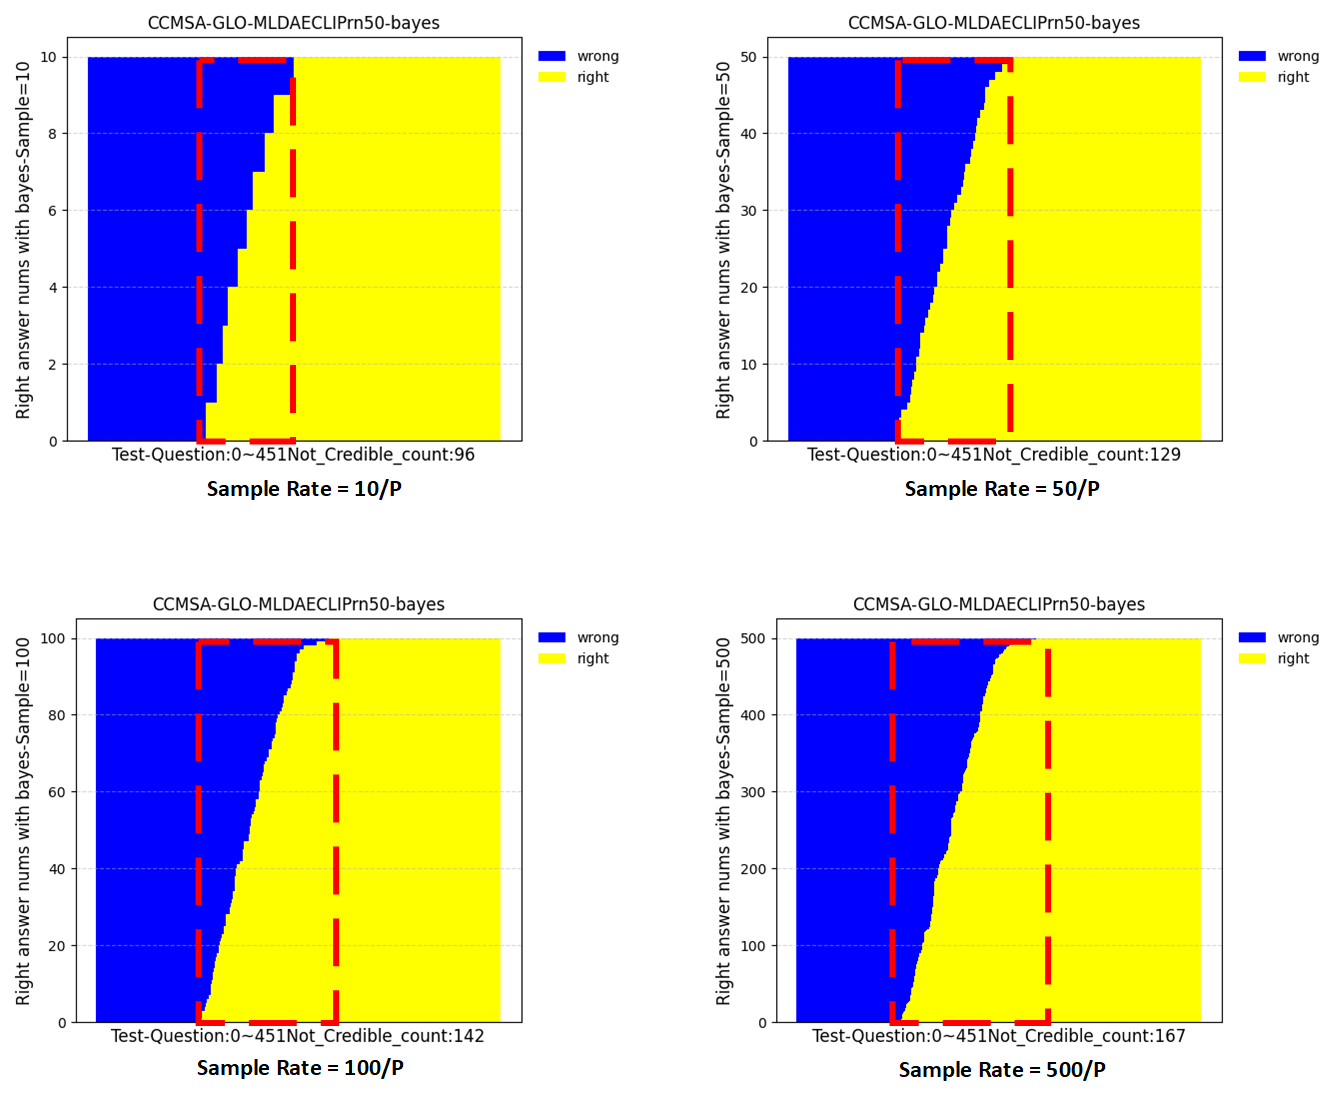
\includegraphics[width=0.8\textwidth]{Fig/myfig/chapter4/sample_sum.png}  %scale = 0.3
	% 添加标签one_DFUAV以及图标题“XXX”,引用某图时使用\ref{xxx},其中xxx就是标签,图编号是自动生成的。
	\caption{\label{sample_sum}采样频率变化与模型不确定估计} 
\end{figure}

% \begin{figure}[htbp]
% 	\begin{minipage}{0.5\linewidth}
% 		\centering	
% 		% 包含当前路径下的Fig文件夹的图片文件
% 		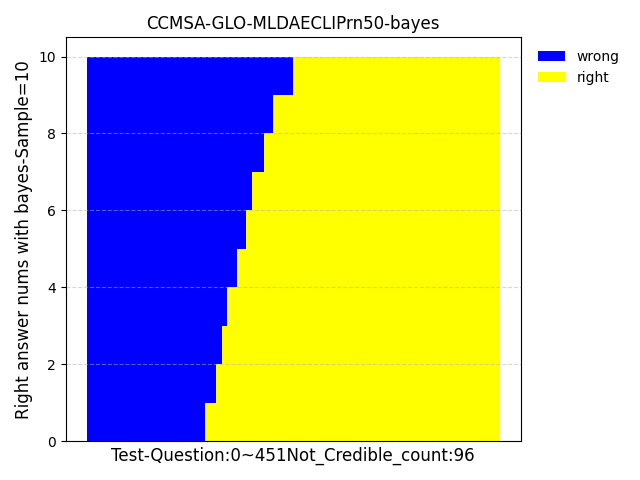
\includegraphics[width=0.8\textwidth]{Fig/myfig/chapter4/sample10.png}  %scale = 0.3
% 		% 添加标签one_DFUAV以及图标题“XXX”,引用某图时使用\ref{xxx},其中xxx就是标签,图编号是自动生成的。
% 		\caption{\label{modal_bayes_sample10}sample = 10} 	
% 	\end{minipage}
% 	% 图片居中(列居中对齐)
% 	\begin{minipage}{0.5\linewidth}
% 		\centering	
% 		% 包含当前路径下的Fig文件夹的图片文件
% 		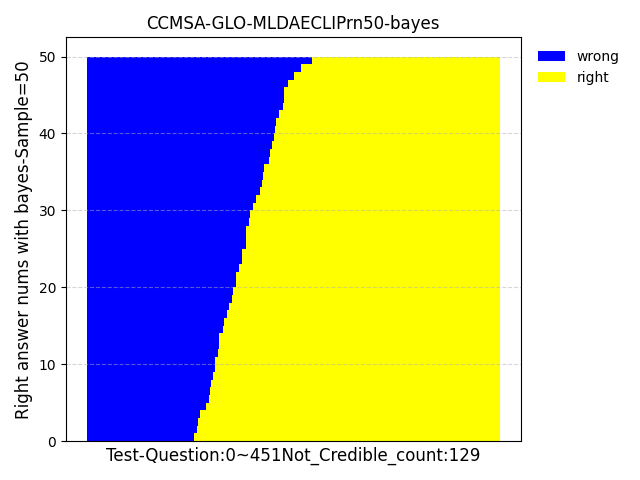
\includegraphics[width=0.8\textwidth]{Fig/myfig/chapter4/sample50.png}  %scale = 0.3
% 		% 添加标签one_DFUAV以及图标题“XXX”,引用某图时使用\ref{xxx},其中xxx就是标签,图编号是自动生成的。
% 		\caption{\label{modal_bayes_sample50}sample = 50} 	
% 	\end{minipage}	
% \end{figure}
% \begin{figure}[htbp]
% 	\begin{minipage}{0.5\linewidth}
% 		\centering	
% 		% 包含当前路径下的Fig文件夹的图片文件
% 		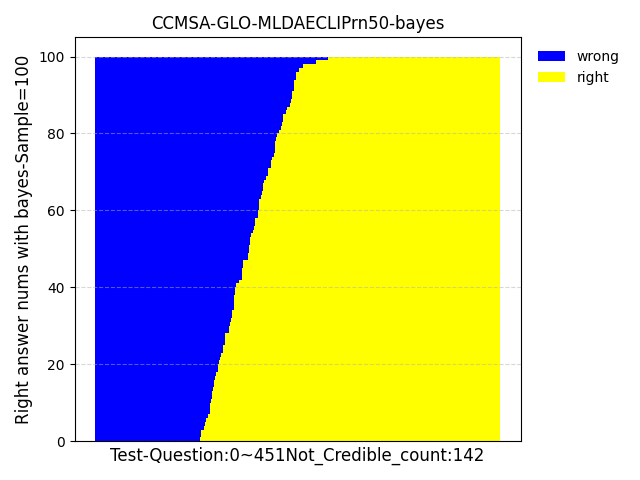
\includegraphics[width=0.8\textwidth]{Fig/myfig/chapter4/sample100.png}  %scale = 0.3
% 		% 添加标签one_DFUAV以及图标题“XXX”,引用某图时使用\ref{xxx},其中xxx就是标签,图编号是自动生成的。
% 		\caption{\label{modal_bayes_sample100}sample = 100} 	
% 	\end{minipage}
% 	% 图片居中(列居中对齐)
% 	\begin{minipage}{0.5\linewidth}
% 		\centering	
% 		% 包含当前路径下的Fig文件夹的图片文件
% 		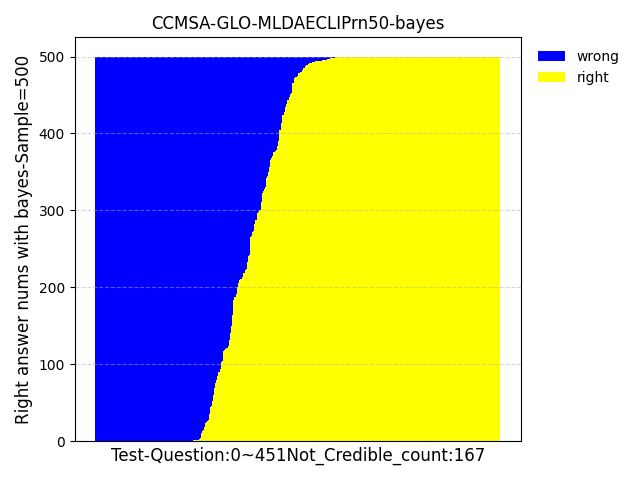
\includegraphics[width=0.8\textwidth]{Fig/myfig/chapter4/sample500.png}  %scale = 0.3
% 		% 添加标签one_DFUAV以及图标题“XXX”,引用某图时使用\ref{xxx},其中xxx就是标签,图编号是自动生成的。
% 		\caption{\label{modal_bayes_sample500}sample = 500} 	
% 	\end{minipage}	
% \end{figure}
%
\begin{table}
	\caption{\label{sample_exm}不同采样率下问答结果的不确定性}
	\centering
	\small % 调整表格字号
	\begin{tabular}{c|ccc}
		\hline Dataset & 采样频率 & 不确定性的问答数U/总问答数A & 回答预测分布的方差 \\
		\hline \multirow{4}{*}{Med-RAD} & 10 & 0.21 & 2639.96 \\
		& 50 & 0.25 & 2656.54 \\
		& 100 & 0.30 & 2711.51 \\
		& 500 & 0.31 & 2758.05 \\
		\hline \multirow{4}{*}{Slake} & 10 & 0.21 & 355.00 \\
		& 50 & 0.24 & 396.82 \\
		& 100 & 0.29 & 401.05 \\
		& 500 & 0.32 & 398.77 \\
		\hline
	\end{tabular}
\end{table}
从图中可以看出,随着采样频率的增大,模型捕获不确定性的能力增强,可以充分捕获当下预测的样本点以及其周围邻域是否有充足的近似样本分布来支撑模型对其结果的确信程度
以及消解对其预测的不确定性。在表\ref{sample_exm}中,可见由于Med-RAD数据集相比SLAKE数据集数据量较少,在分类空间上缺少"支撑样本",从而导致整体预测的不确定性,也就是预测回答分布的方差较大,并随着采样频率的增大,这个数值也会增大。
这一实验一定程度上解释了分类模型的不确定性和输入样本分布之间的关联,以及通过增大采样频率,可以增强模型预测不确定性的能力。但同时从图中也可以看出,由采样定理
这种增强并不是线性增长,而是逐渐接近一个极限值。

%这个极限值理想化即为采样-不确定性极限。


\subsection{拒绝分类实验}
从理论上来说,由于预测不确定是贝叶斯神经网络最突出的优点之一,预测不确定性越高,说明网络对预测结果的把握程度越低,所以对于不确定性过高的预测,网络往往可以通过拒绝分类的形式,即不给出分类结果,
从而提高模型分类的准确性和可靠程度。在实际的医学问答等具有风险性的情景中,当面对具有高不确定的诊断场合时,医生也会拒绝给出确切的答复,并通过其他手段继续收集信息以降低不确定性后再给出确诊意见,
从而防止漏诊、误诊以及误治等具有极大事故风险的情况出现。

为了验证拒绝分类这一想法的可行性,本文利用MEMSA网络以及用于对其进行分类预测的BMLP探究模型拒绝对不确定性高的类别进行预测是否能够提高模型整体的准确率。在实验前,首先需要一种具体计算样本预测不确定性的方法。由于BNN的权值为
变分的形式,所以其预测输出也是一种变分分布。Kwon等人\cite{kwon2020uncertainty}和Shridhar等人\cite{shridhar2018uncertainty}提出通过计算变分预测分布$q\left(y^* \mid x^*\right)$的方差来度量预测不确定性:
\begin{equation}
	\label{varpredict}
	\begin{aligned}
	\operatorname{Var}_{q\left(y^* \mid x^*\right)}\left(y^*\right) & =\int\left[\operatorname{diag}\left\{E_{p\left(y^* \mid x^*, w\right)}\left(y^*\right)\right\}-E_{p\left(y^* \mid x^*, w\right)}\left(y^*\right)^{\otimes 2}\right] q(w) d w \\
	& +\int\left\{E_{p\left(y^* \mid x^*, w\right)}\left(y^*\right)-E_{q\left(y^* \mid x^*\right)}\left(y^*\right)\right\}^{\otimes 2} q(w) d w
	\end{aligned}
\end{equation}
其中$v^{\otimes 2} = vv^{T}$,$x^{*}$和$y^{*}$分别是测试样本以及预测输出,$p\left(y^* \mid x^*, w\right)$表示给定$w$下网络的预测,$q(w)$表示权值的变分分布,$diag(v)$是以向量v为对角线元素的
对角矩阵。公式\eqref{varpredict}通常难以精确计算,但该式子仍可以通过蒙特卡洛方法进行近似\cite{kwon2020uncertainty}:
\begin{equation}
	\label{}
	\operatorname{Var}_{q\left(y^* \mid x^*\right)}\left(y^*\right)=\frac{1}{T} \sum_{t=1}^T \operatorname{diag}\left(\hat{p}_t\right)-\hat{p}_t \hat{p}_t^T+\frac{1}{T} \sum_{t=1}^T\left(\hat{p}_t-\bar{p}\right)\left(\hat{p}_t-\bar{p}\right)^T
\end{equation}
其中T为蒙特卡洛采样次数、$\hat{p}_t$代表第t次采样的网络输出的预测概率、$\bar{p}$是所有$\hat{p}_t$的均值,即$\bar{p}=\sum_{t=1}^T \hat{p}_t / T$。在Kwon等人\cite{kwon2020uncertainty}的推导中,公式右边第一项为偶然不确定性或数据不确定性,第二项为认知不确定性或模型不确定性。
偶然不确定性描述观测数据中固有的噪声,这是一项无法消除和避免的误差。即时收集更多的数据,只要采集方式或数据的分布形式不变,也无法降低偶然不确定性。认知不确定性描述的是训练模型中的权重参数时产生的不确定性,只与模型网络自身有关。
认知不确定性反映的是模型缺乏与样本相对应的知识或先验。例如,对于来源于数据稀疏区域或者远离训练集的测试点,模型的认知不确定性就会显著增加\cite{kendall2017uncertainties}。所以通过收集更多的数据训练模型,可以减少认知不确定性。Shridhar等人\cite{shridhar2018uncertainty}的实验表明,分类准确性和认知不确定性之间呈
负相关的关系,即分类准确性随着认知不确定性降低而提高。Shridhar等人\cite{shridhar2018uncertainty}还证明偶然不确定性取决于数据集而不是模型,同一个数据集在不同模型下具有相同的偶然不确定性。因此,本文将认知不确定性作为衡量模型预测不确定性高低的主要指标。

本文设计的拒绝分类实验过程如下:训练完成后固定网络参数进行测试,测试时,首先对模型进行10次蒙特卡洛采样,计算所有样本的认知不确定性。之后对这些样本按照认知不确定性的大小进行排序,并按照不同的拒绝比例(例如$0\%$、$10\%$、$25\%$、$50\%$)将不确定性高的样本从舍弃,相当于BNNs拒绝对这些样本进行分类,之后重新计算拒绝分类后
的预测准确率。
% ,如图\ref{reject_sum}所示。
% \begin{figure}[htbp]
% 	% 图片居中(列居中对齐)
% 	\centering	
% 	% 包含当前路径下的Fig文件夹的图片文件
% 	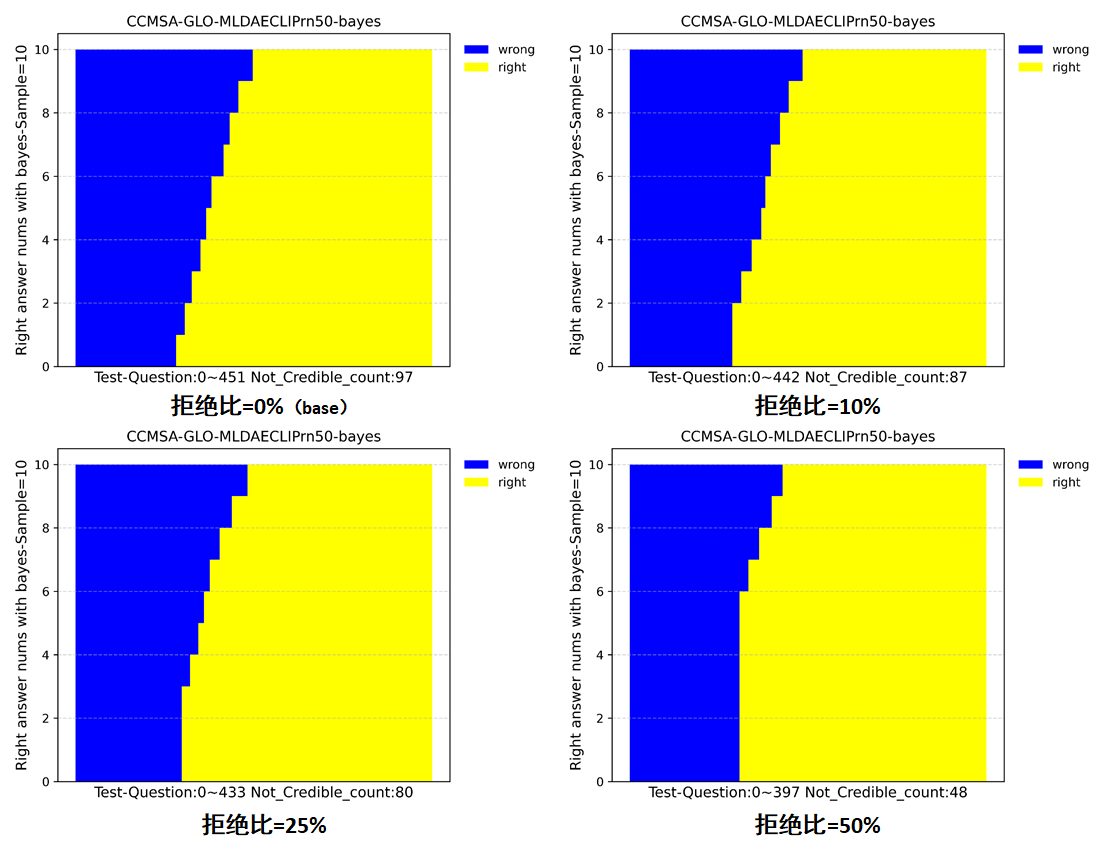
\includegraphics[width=0.8\textwidth]{Fig/myfig/chapter4/reject_sum.png}  %scale = 0.3
% 	% 添加标签one_DFUAV以及图标题“XXX”,引用某图时使用\ref{xxx},其中xxx就是标签,图编号是自动生成的。
% 	\caption{\label{reject_sum}不同拒绝比下的模型表现} 
% \end{figure}

表\ref{reject_exm}显示了模型按所设定的不同比例拒绝高认知不确定样本后的问答准确率。当拒绝比例为$n \%$时,代表$n \%$认知不确定性值最高的样本被拒绝分类。可以看到,当网络拒绝分类部分预测不确定性高的样本之后,在开放式问答(Open)和封闭式问答(Close)上的回答准确率均有提升;
可以看到,当以百分之50的拒绝比例拒绝高认知不确定性样本时,网络在Med-RAD、Slake这两个数据集上的总问答准确率分别提高到了73.8\%和81.0\%,接近甚至超越了在没有引入不确定估计时模型的预测水平,在该数据集上也是一个相当高的准确率。
且对于数据不确定性较高的小样本数据集Med-RAD,拒绝比例越大,准确率的增长率越大,提升幅度也越明显。以上结果说明,被拒绝分类的样本中大部分为容易分类错误的样本,同时也解释了拒绝分类可以升Med-VQA模型问答性能。
\begin{table}
	\caption{\label{reject_exm}拒绝分类实验结果}
	\centering
	\small % 调整表格字号
	\begin{tabular}{c|c|ccccc}
		\hline Dataset & 拒绝比例 & Open & Close & Overall & Growth rate & U/A \\
		\hline \multirow{4}{*}{Med-RAD} & 0 \%& 49.7 \%& 74.6 \%& 64.7 \%& X& 0.188 \\
		& 10 \%& 51.3 \%& 75.8 \%& 66.4 \%& 0.8 \% & 0.180 \\
		& 25 \%& 58.7 \%& 76.5 \%& 70.4 \%& 1.3 \% & 0.161 \\
		& 50 \%& 65.0 \%& 77.7 \%& 73.8 \%& 2.8 \% & 0.137 \\
		\hline \multirow{4}{*}{Slake} & 0 \%& 74.0 \%& 79.1 \%& 76.0 \%& X& 0.187 \\
		& 10 \%& 76.0 \%& 79.4 \%& 77.4 \%& 1.4 \% & 0.177 \\
		& 25 \%& 79.1 \%& 79.4 \%& 79.2 \%& 1.8 \% & 0.154 \\
		& 50 \%& 82.1 \%& 79.6 \%& 81.0 \%& 1.8 \% & 0.139 \\
		\hline
	\end{tabular}
\end{table}

综上所述,认知不确定性可以在一定程度上反映样本被错分类的可能性,认知不确定性高的样本中,错分类的样本占多数,说明模型对容易错分类的样本会具有较大的认知不确定性。因此,贝叶斯神经网络模型
可以通过拒绝认知不确定性高的样本进行分类来提高模型的准确性,同时尽可能避免了错分类的产生,可以说BNNs的加入提高了整个医学视觉问答系统的性能和可靠性。

\subsection{带不确定性估计的问答样例}
当设定BMLP的采样频率(sample)取10的时候,模型不确定性估计样例如图\ref{qademo}所示,针对Q1提问,当所有的采样子网络预测结果都指向一个答案标签(Right upper lobe)时,依据上文提到的贝叶斯不确定性估计相关原理\cite{blundell2015weight},此估计方差和标准差为0
我们认为这个答案是具有低不确定性的,具有更好的可靠性。
\begin{figure}[htbp]
	% 图片居中(列居中对齐)
	\centering	
	% 包含当前路径下的Fig文件夹的图片文件
	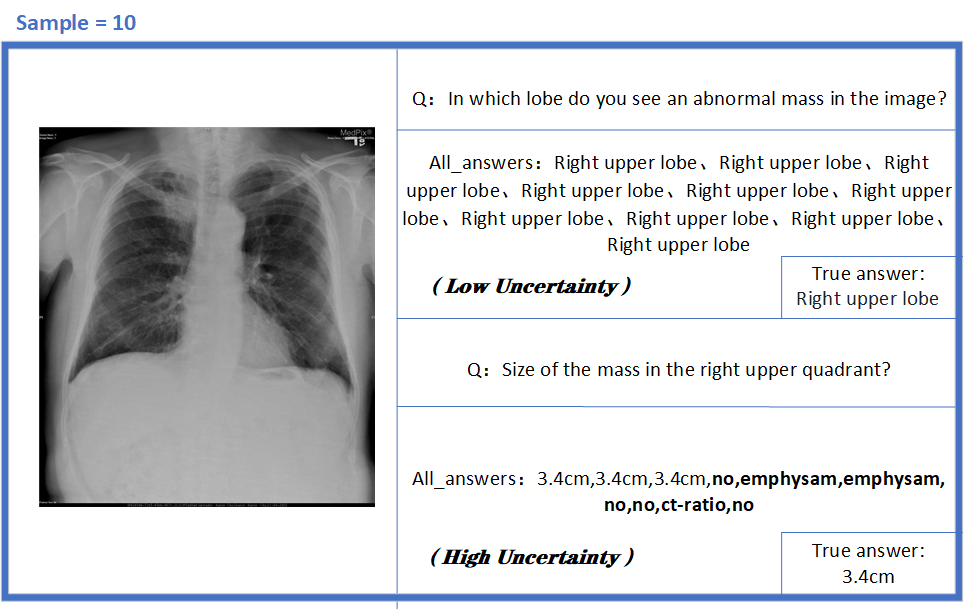
\includegraphics[width=0.8\textwidth]{Fig/myfig/chapter4/qadamo.png}  %scale = 0.3
	% 添加标签one_DFUAV以及图标题“XXX”,引用某图时使用\ref{xxx},其中xxx就是标签,图编号是自动生成的。
	\caption{\label{qademo}采样率为10时带不确定性问答样例} 
\end{figure}

对于Q2提问,不同子网络给出了不同的答案,而且呈现零散分布的态势,具有极高的方差和标准差,所以是具有高不确定性的答案。即使其中包含了正确的答案,但我们通过不确定性预测认为这个答案是
不可靠的,因为按先验分布对样本点以及其周围邻域采样时会出现影响结果的样本点,说明该预测是一种在超平面上,也就是对边界样本的预测,模型对该类型预测往往具有极高错分类的概率,也就是这时同结构的点估计网络下对其的预测往往是不准确的,这种答案不具备参考性。
可见,基于BNNs搭建的BMLP可以知晓自己预测时的样本分布情况,从而预测出其结果的不确定性,这种预测优势是传统点估计网络所无法具备的。BMLP也模仿了人在事前对信息(样本分布以及先验)掌握不充分的情况下做出预测时会给出的一种不确定,不肯定评估,这种不确定性评估虽然不具备信息增强的能力,但可以帮助我们在某些场合进行预测时规避掉重大的风险,从而步步为营,
以较高质量完成后续任务以及目标。

\section{本章小结}
本章首先介绍了贝叶斯神经网络的原理、结构以及该结构和不确定估计之间的关系,然后对网络中局部使用贝叶斯神经网络和全局使用贝叶斯神经网络进行了简单的阐述和定性分析,接着网络搭建部分,
先后介绍了用于医学视觉问答网络中的BNNs结构以及BNN中先验和后验的选择依据和技巧,紧接着网络训练部分详解了用于BNN训练的贝叶斯反向传播算法以及网络如何进行输出和预测以及与不确定性的关系,介绍了模型的参数
构成与复杂度。最后通过模型问答性能实验、采样与不确定性的关系实验和拒绝分类实验验证了BNNs相比传统点估计网络所具有的防止过拟合、获得预测分布以及不确定性以及通过拒绝分类的形式可以提升模型
性能以及防止错分类等等优势。

综上,本章验证了通过将贝叶斯神经网络引入具有风险性的医学视觉问答场景不但可以提高模型性能、提高模型在缺少数据样本时的鲁棒性和防止过拟合,还可以通过不确定估计和拒绝分类的形式,极大地提高了模型甚至
医学视觉问答系统的可靠性,具备相当的实用价值。



